\documentclass[activite]{thedocument}
\usepackage{texmaths-boxes}
\startdatakeys
\source{}
\cycle{}
\competencesDuSocle{}
\connaissancesRequises{}
\competencesTravaillees{}
\enddatakeys
\begin{document}
    \begin{center}
        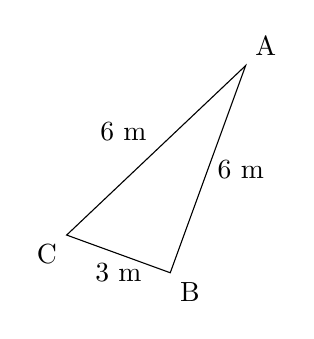
\begin{tikzpicture}[rotate=-20,scale=0.7]
            \coordinate[label=above right:A](A)at(2,4);
            \coordinate[label=below left:C](C)at(0,0);
            \coordinate[label=below right:B](B)at(2,0);
            \path(A)--(B)node[midway,right]{6 m};
            \path(A)--(C)node[midway,above left]{6 m};
            \path(C)--(B)node[midway,below]{3 m};
            \draw(A)--(B)--(C)--cycle;
        \end{tikzpicture}
    \end{center}\vskip50pt
    {\centering\TableauRaisonnement scale=200pt;\par}
\end{document}